\documentclass [12pt]{article}   %\makeatletter
\usepackage{graphicx}
\usepackage{epstopdf}
\usepackage{subfigure}
\usepackage{amssymb, amsmath}
\usepackage{amsfonts}
\usepackage[compress]{cite}
\usepackage{float}
\epstopdfsetup{update}
\topmargin -1.5cm       
 \oddsidemargin -0.04cm   
 \evensidemargin -0.04cm  
 \textwidth 16.59cm
 \textheight 21.94cm 


\begin{document}
\begin{center}
{\bf \Large ECE412 - Digital Control \& Digital Filters}

\smallskip
{\bf \large Digital Filter Transformation}

\end{center}

\renewcommand{\baselinestretch}{1}\small\normalsize
\medskip
There are two approaches to the design of digital filters of bandpass, highpass, and bandstop types.
\begin{enumerate}
	\item Design an analog lowpass filter, apply the frequency band transformations in analog domain, and then map the relevant filter to a digital filter 
	
	\medskip
	{\bf \underline{Disadvantage}} 
	
	\medskip
	Due to aliasing problem inherent in the use of impulse invariant technique a bandpass or highpass filter cannot be transformed.
	\item Design an analog lowpass filter, map it to a digital filter, and then apply frequency band transformations in digital domain to obtain the desired digital filter.
	
	\smallskip
	In this handout we introduce the second approach by defining several transformations to map a LPF to a LPF, BPF, and HPF with given specifications.
\end{enumerate}

\medskip
Define a mapping from the $z$-plane to the $\tilde{z}$-plane of the form
\begin{equation}
	z^{-1}=f(\tilde{z}^{-1})
\end{equation}
such that the transfer function
\begin{equation}
	H(z^{-1}) \overset{\textnormal{mapped}}{\longrightarrow} G(\tilde{z}^{-1})
\end{equation}
Conditions for this mapping are
\begin{enumerate}
	\item $f(\cdot)$ is real and rational.
	\item $f(\cdot)$ must produce stable $G(\tilde{z}^{-1})$ from $H(z^{-1})$ i.e. the interior of the unit circle in the $z$-plane must be mapped to the interior of the unit circle in the $\tilde{z}$-plane. 
	\item $|f(\tilde{z}^{-1})| = 1$, $|z^{-1}| = 1$
\end{enumerate}
A class of transformation for mapping a LPF to another LPF with different frequency characteristics or to a HPF, has a general form of
\begin{equation}
	f(\tilde{z}^{-1}) = \frac{a_0+a_1\tilde{z}^{-1}}{1+b_1 \tilde{z}^{-1}}
\end{equation}
\begin{figure}[H]
	\centering
	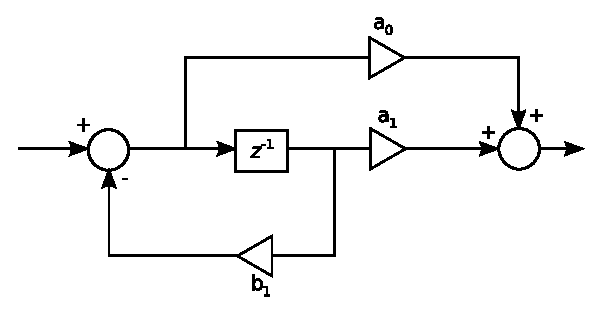
\includegraphics[width=3.5in]{transformation.eps}
	\label{fig:transformation}
\end{figure}
\begin{enumerate}
	\item \underline{Lowpass to Lowpass mapping} 
	
	The transformation
	\begin{equation}
		z^{-1} = f(\tilde{z}^{-1}) = \frac{\tilde{z}^{-1}-\alpha}{1-\alpha\tilde{z}^{-1}}
	\end{equation}
	\begin{figure}[H]
		\centering
		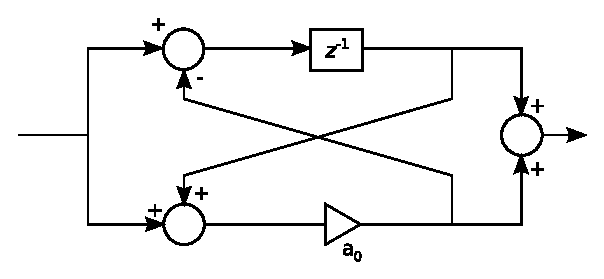
\includegraphics[width=3.5in]{transformation1.eps}
		\label{fig:transformation1}
	\end{figure}
	which satisfies the above conditions can be used to map a LPF to another LPF. Let $z=e^{j\Omega T}$ and $\tilde{z} = e^{j\tilde{\Omega}T}$. Then the relationship between the frequencies $\Omega$ and $\tilde{\Omega}$ is
	\begin{equation}
		\Omega = \frac{2}{T} \tan^{-1}(K \tan \frac{\tilde{\Omega T}}{2}),~K = \frac{1+\alpha}{1-\alpha}
	\end{equation}
	where $\alpha$ can be obtained based upon the cutoff frequency of the transformed filter.
	\bigskip
	\begin{figure}[H]
		\begin{center}
			\mbox{
				\subfigure[Passband and stopband of the original LPF on the unit circle]{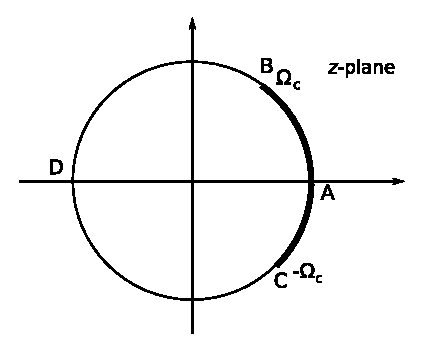
\includegraphics[width=2.75in]{LPForig.eps}} \quad
				\subfigure[Passband and stopband of the mapped LPF on the unit circle]{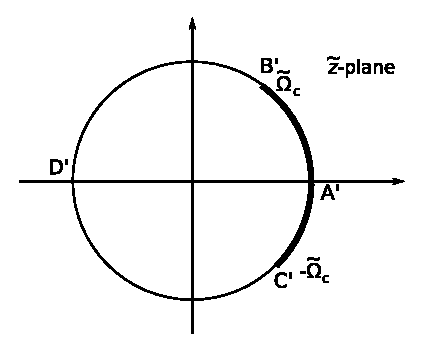
\includegraphics[width=2.75in]{LPFmapped.eps}}
			}
		\end{center}
	\end{figure}
	\newpage
	\item \underline{Lowpass to Highpass mapping}
	
	We desire to map
	\begin{figure}[H]
		\centering
		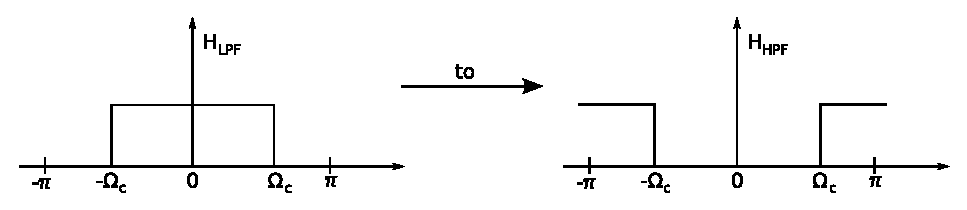
\includegraphics[width=5.5in]{LPFHPFmap.eps}
		\label{fig:transformation2}
	\end{figure}
	On the unit circle we must rotate the frequency band.
	\begin{figure}[H]
		\centering
		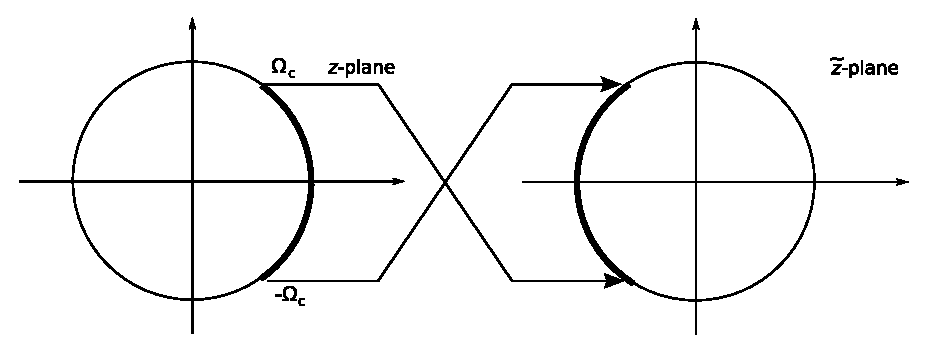
\includegraphics[width=5in]{LPFHPFunitmap.eps}
		\label{fig:transformation2unit}
	\end{figure}
	Thus, the mapping is
	\begin{equation}
		z^{-1} \longrightarrow -\tilde{z}^{-1},~z^{-1} \longrightarrow -z^{-1}
	\end{equation}
	or in general
	\begin{equation}
		z^{-1} \longrightarrow \frac{-(\tilde{z}^{-1}+\alpha)}{1+\alpha\tilde{z}^{-1}}
	\end{equation}
	The cutoff frequency of the HPF is related to that of LPF by 
	\begin{equation}
		\Omega_{c_{HP}} + \Omega_{c_{LP}}=\frac{\pi}{T}~ \textnormal{(normalized case)}
	\end{equation}
	\begin{figure}[H]
		\centering
		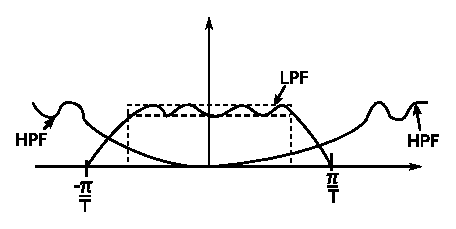
\includegraphics[width=4in]{LPFHPFnorm.eps}
		\label{fig:transformation2norm}
	\end{figure}
	\newpage
	\item \underline{Lowpass to Bandpass Mapping}
	
	We desire to map
	\begin{figure}[H]
		\centering
		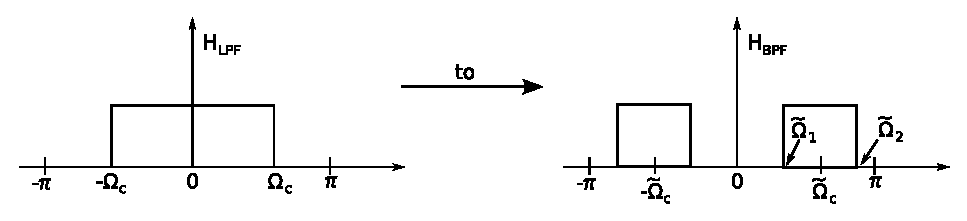
\includegraphics[width=5.5in]{LPFBPFmap.eps}
		\label{fig:transformation3}
	\end{figure}
	Note that since every point in LPF characteristics is mapped to two points in that of the BPF, we need a 2nd order mapping i.e.
	\begin{equation}
		z^{-1} = f(\tilde{z}^{-1}) = \frac{a_0 + a_1 \tilde{z}^{-1}+a_2 \tilde{z}^{-2}}{b_0 + b_1 \tilde{z}^{-1}+b_2 \tilde{z}^{-2}}
	\end{equation}
	\begin{figure}[H]
		\centering
		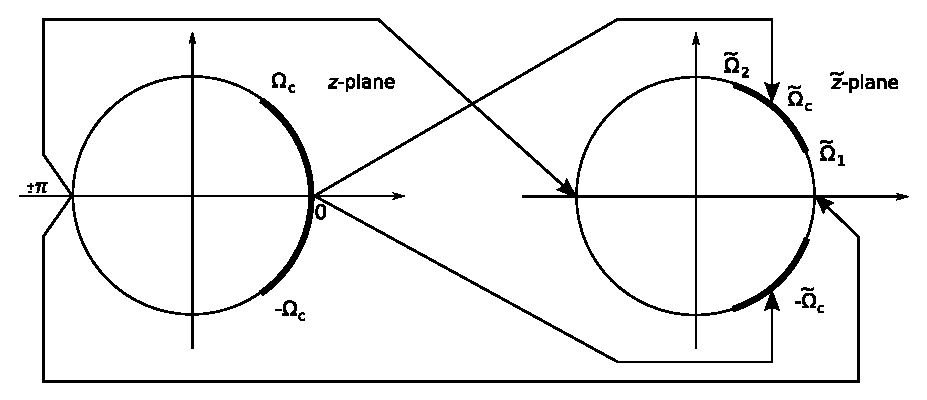
\includegraphics[width=5in]{LPFBPFunitmap.eps}
		\label{fig:transformation3unit}
	\end{figure}
	It can be shown that the mapping which satisfies the above mentioned conditions will have a form
	\begin{equation}
		z^{-1}=f(\tilde{z}^{-1})=-\left[\frac{a_0+a_1 \tilde{z}^{-1} + a_2 \tilde{z}^{-2}}{a_2 + a_1 \tilde{z}^{-1}+a_0 \tilde{z}^{-2}}\right]
	\end{equation}
	or in a more useful form
	\begin{equation}
		z^{-1} = f(\tilde{z}^{-1}) = -\left[\frac{\tilde{z}^{-2} - \frac{2\alpha K}{K + 1}\tilde{z}^{-1} + \frac{K-1}{K+1}}{\frac{K-1}{K+1}\tilde{z}^{-2}-\frac{2\alpha K}{K+1}\tilde{z}^{-1}+1}\right]
	\end{equation}
	where
	\begin{eqnarray} \nonumber
		K & = & \frac{a_0 + a_2}{a_0 - a_2} \\
		  & = & \tan \frac{\Omega_c T}{2} \left[\cot \left[\left(\frac{\tilde{\Omega}_2 - \tilde{\Omega}_1}{2}\right)T\right]\right]
	\end{eqnarray}
	and $\alpha = \cos \tilde{\Omega}_0,~T= -\frac{a_1}{a_0+a_2}$, where $\tan \frac{\tilde{\Omega}_1-\tilde{\Omega}_2 T}{2} = \tan \frac{\Omega_c T}{2}$
	
	\medskip
	\underline{Special Cases:}
	
	\medskip
	\begin{enumerate}
		\item $K = 1 \longrightarrow \frac{\tilde{\Omega}_2-\tilde{\Omega}_1}{2},~T=\frac{\pi}{2}-\Omega_c \frac{T}{\lambda}$ i.e. the BW is constant and we have a variable frequency filter (tracking filter) since we can track the center frequency.
		\item $\alpha = 0 \longrightarrow \tilde{\Omega}_0T = \frac{\pi}{2} \longrightarrow \tilde{\Omega}_0 = \frac{\pi}{2T}$ or $\frac{\tilde{\Omega}_1 + \tilde{\Omega}_2}{2}=\frac{\pi}{2T}$ i.e. we can vary the BW and the center frequency is fixed. This is used in ``vestigial sideband''.
		\item \begin{equation}
		\left.\begin{array}{c} K = 1 \\ \alpha = 0 \end{array}\right]\longrightarrow \begin{array}{c c} \tilde{\Omega}_2 - \tilde{\Omega}_1 = \frac{\pi}{T} - \Omega_c & \tilde{\Omega}_2 = \frac{\pi}{T} - \frac{\Omega_c}{2} \\ \tilde{\Omega}_2 + \tilde{\Omega}_1 = \frac{\pi}{T} & \tilde{\Omega}_1 = \frac{\Omega_c}{2} \end{array}\end{equation}
		Thus, the mapping is
		\begin{equation}
			z^{-1} \longrightarrow -\tilde{z}^{-1}.
		\end{equation}
	\end{enumerate}
\end{enumerate}
\begin{figure}[H]
	\centering
	\includegraphics[width=3.75in]{LPFBPFmap2.eps}
	\label{fig:transformation32}
\end{figure}

\end{document}
